\label{chap:mecanique}
\begin{figure}[H]
    \centering
    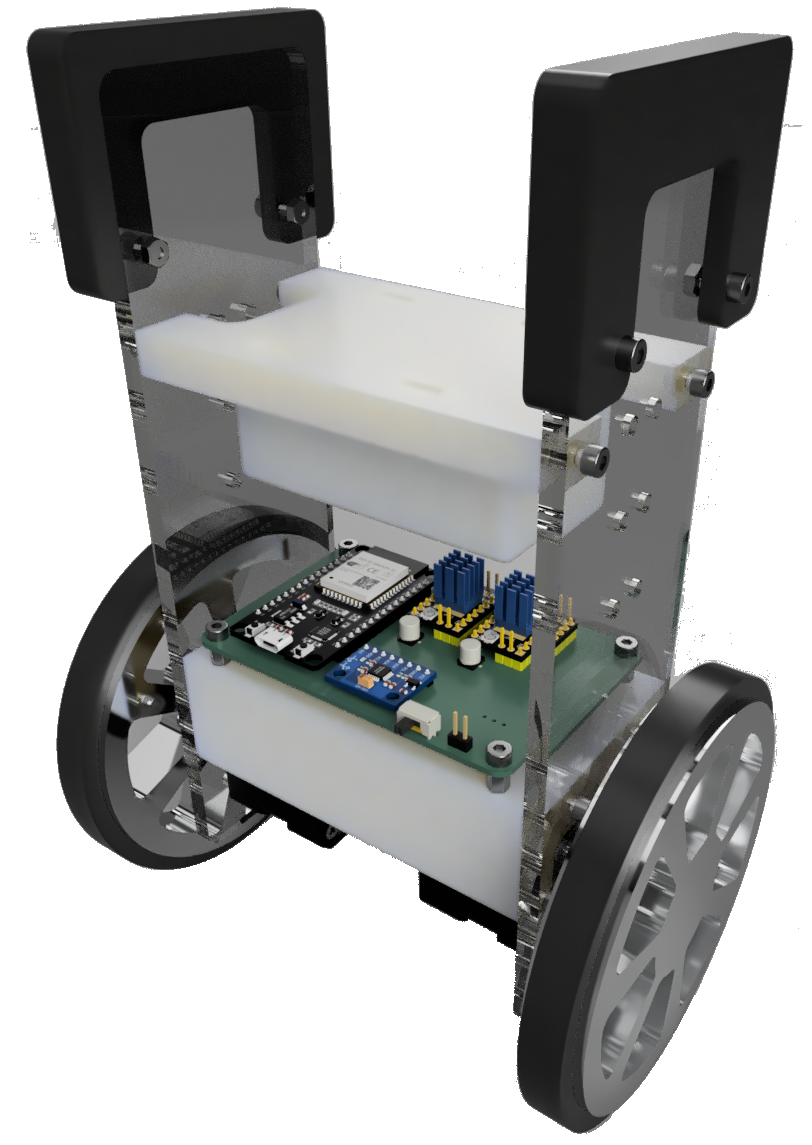
\includegraphics[width=0.8\textwidth]{assets/figures/meca_raytracing.png}
    \caption{Maquette 3D, raytracée}
    \label{fig:meca_raytraced}
\end{figure}

Une fois le principe physique expliquée, il est temps de réaliser la maquette. Le but ici est de tenir compte des reflexions faites durant la partie théorique.

Dans ce chapitre, l'entiereté de la conception mécanique de la maquette sera traitée en commençant par les outils utilisés, en traitant ensuite des contraintes mécaniques connues.

Finalement, une rapide instruction de montage sera présentée.

L'ensemble des dessins mécanique se trouvent à l'annexe \ref{annexe:dessins_mecaniques}. De plus, les fichiers 3D des pièces se trouvent également sur le Git indiqué en annexe \ref{annexe:git}.

\section{Méthode et outils}
\subsection{Logiciels}

La conception mécanique du robot a été réalisée à l'aide du logiciel Fusion360 de Autocad. Cette étape a permis de modéliser l'ensemble des composants du robot avant leur fabrication, de vérifier leur intégration ainsi que d'anticiper les éventuels problèmes d'assemblage.

L'utilisation d'un modèle tridimensionnel présente plusieurs avantages. Elle permet notamment de contrôler les dimensions de l'ensemble, de vérifier les interfaces entre les différents composants, d'optimiser la répartition des masses et de préparer la fabrication des différentes pièces.

Le PCB ayant été réalisé en premier, ce deriner a été importé dans le modèle afin de pouvoir l'intégrer directement au dessin 3D.
\subsection{Outillage}

Essentiellement, le robot est constitué de pièces imprimées en 3D ainsi que de pièces découpées au laser. Divers éléments d'assemblage (vis, colonnettes, écrous, etc.) proviennent du MakeLab ou de l'atelier mécanique.

Les pneus ainsi que les protections anti-chutes ont été imprimé en TPU, un filament flexible afin d'améliorer l'adhérance et amortir l'impact d'une éventuelle chute.

Le tableau \ref{tab:machines} répertorie l'ensemble des machines utilisées pour la fabrication de la maquette.

\begin{table}[H]
\centering
\begin{tabular}{|c|p{6cm}|c|}
\hline
\textbf{Machine} & \textbf{Emplacement} & \textbf{Technologie} \\
\hline
Prusa Core One & MakeLab & \acrshort{fdm} \\
\hline
CNC 3 axes & Centre de formation des polymécaniciens, Payerne & Usinage CNC \\
\hline
Découpeuse laser & MakeLab & Découpe laser \\
\hline
BambuLab V1 & MakeLab & \acrshort{fdm}, TPU \\
\hline
\end{tabular}
\caption{Machines utilisées pour la fabrication de la maquette}
\label{tab:machines}
\end{table}

\section{Contraintes mécaniques}

Avant de débuter la conception du châssis, plusieurs contraintes mécaniques ont été identifiées soit par le cahier des charges, soit par le chapitre \ref{chap:principe_physique}.

Les principales contraintes sont les suivantes :

\begin{itemize}
    
    \item assurer une rigidité suffisante afin de limiter les déformations du châssis ;
    \item assurer un positionnement du centre de gravité "variable" ;
    \item limiter la masse totale du robot ; 
    \item garantir un encombrement réduit tout en conservant un accès aisé aux composants ;
    \item permettre un montage et un démontage simples des différents éléments ;
    \item prévoir un passage des câbles limitant les risques d'arrachement ou de frottement avec les parties mobiles.
\end{itemize}

Ces contraintes ont servi de fil conducteur durant toute la phase de conception mécanique.


\subsection{Centre de gravité}

Le centre de gravité constitue un élément essentiel dans la conception d'un robot auto-équilibrant. Contrairement à un robot classique, la stabilité dépend directement de la position de la masse par rapport à l'axe des roues.

Un centre de gravité situé plus haut augmente le bras de levier entre la masse et les roues. Le robot bascule alors plus lentement, ce qui laisse davantage de temps au correcteur pour réagir. En revanche, cette configuration nécessite un déplacement plus important des roues pour maintenir l'équilibre.

À l'inverse, un centre de gravité trop bas rend le système beaucoup plus réactif mais également plus difficile à stabiliser, les variations d'angle étant plus rapides.

C'est pour cette raison que plusieurs perçage ont été réalisés sur les plaques en PVC se situant sur les côtés, de cette manière, la batterie peut être déplacée afin de modifier les caractéristiques du robot.

\subsection{Rigidité}

Le châssis doit présenter une rigidité suffisante afin que les mouvements du robot correspondent fidèlement aux mesures fournies par l'unité de mesure inertielle (IMU).

Une structure trop flexible pourrait engendrer des vibrations ou des déformations susceptibles de perturber les mesures d'accélération et de vitesse angulaire, ce qui dégraderait les performances du système d'équilibrage.
\subsection{Masse}

La masse du robot influence directement le couple que doivent fournir les moteurs ainsi que la consommation électrique.

Dans cette optique, les matériaux utilisés dans la fabrication du châssis ne sont pas massique, à l'exception des roues, (voir\ref{subsection:roues}).

\subsection{Encombrement}

Les dimensions du robot ayant été indiquées par le cahier des charges, voici les dimensions obtenues.

156x143x248mm

L'implantation des différents modules a également été étudiée afin de faciliter l'assemblage, la maintenance ainsi que le passage des câbles. Une attention particulière a été portée à l'accessibilité des principaux éléments, notamment la batterie, le switch d'alimentation et les connecteurs.

\subsection{Roues}
\label{subsection:roues}

Le choix des roues joue un rôle important dans le comportement dynamique du robot. Leur diamètre détermine notamment la vitesse linéaire obtenue pour une vitesse de rotation donnée des moteurs, tandis que leur masse influence directement leur moment d'inertie.

Une roue présentant un moment d'inertie élevé nécessite davantage de couple pour accélérer ou ralentir. Cette caractéristique peut modifier la réactivité du système d'équilibrage et influencer les performances de la régulation.

Afin d'évaluer expérimentalement cet effet, deux jeux de roues de géométrie identique ont été réalisés : un premier en aluminium et un second en plastique PLA. Les roues peuvent être interchangeées sans modification de la structure du robot, ce qui permet de comparer directement l'influence de leur masse et de leur moment d'inertie sur le comportement du système.

\section{Assemblage}
Le chassis est assemblé moyennant des vis, écrous et inserts M3.

\section{Caractéristiques}


\begin{figure}[H]
    \centering
    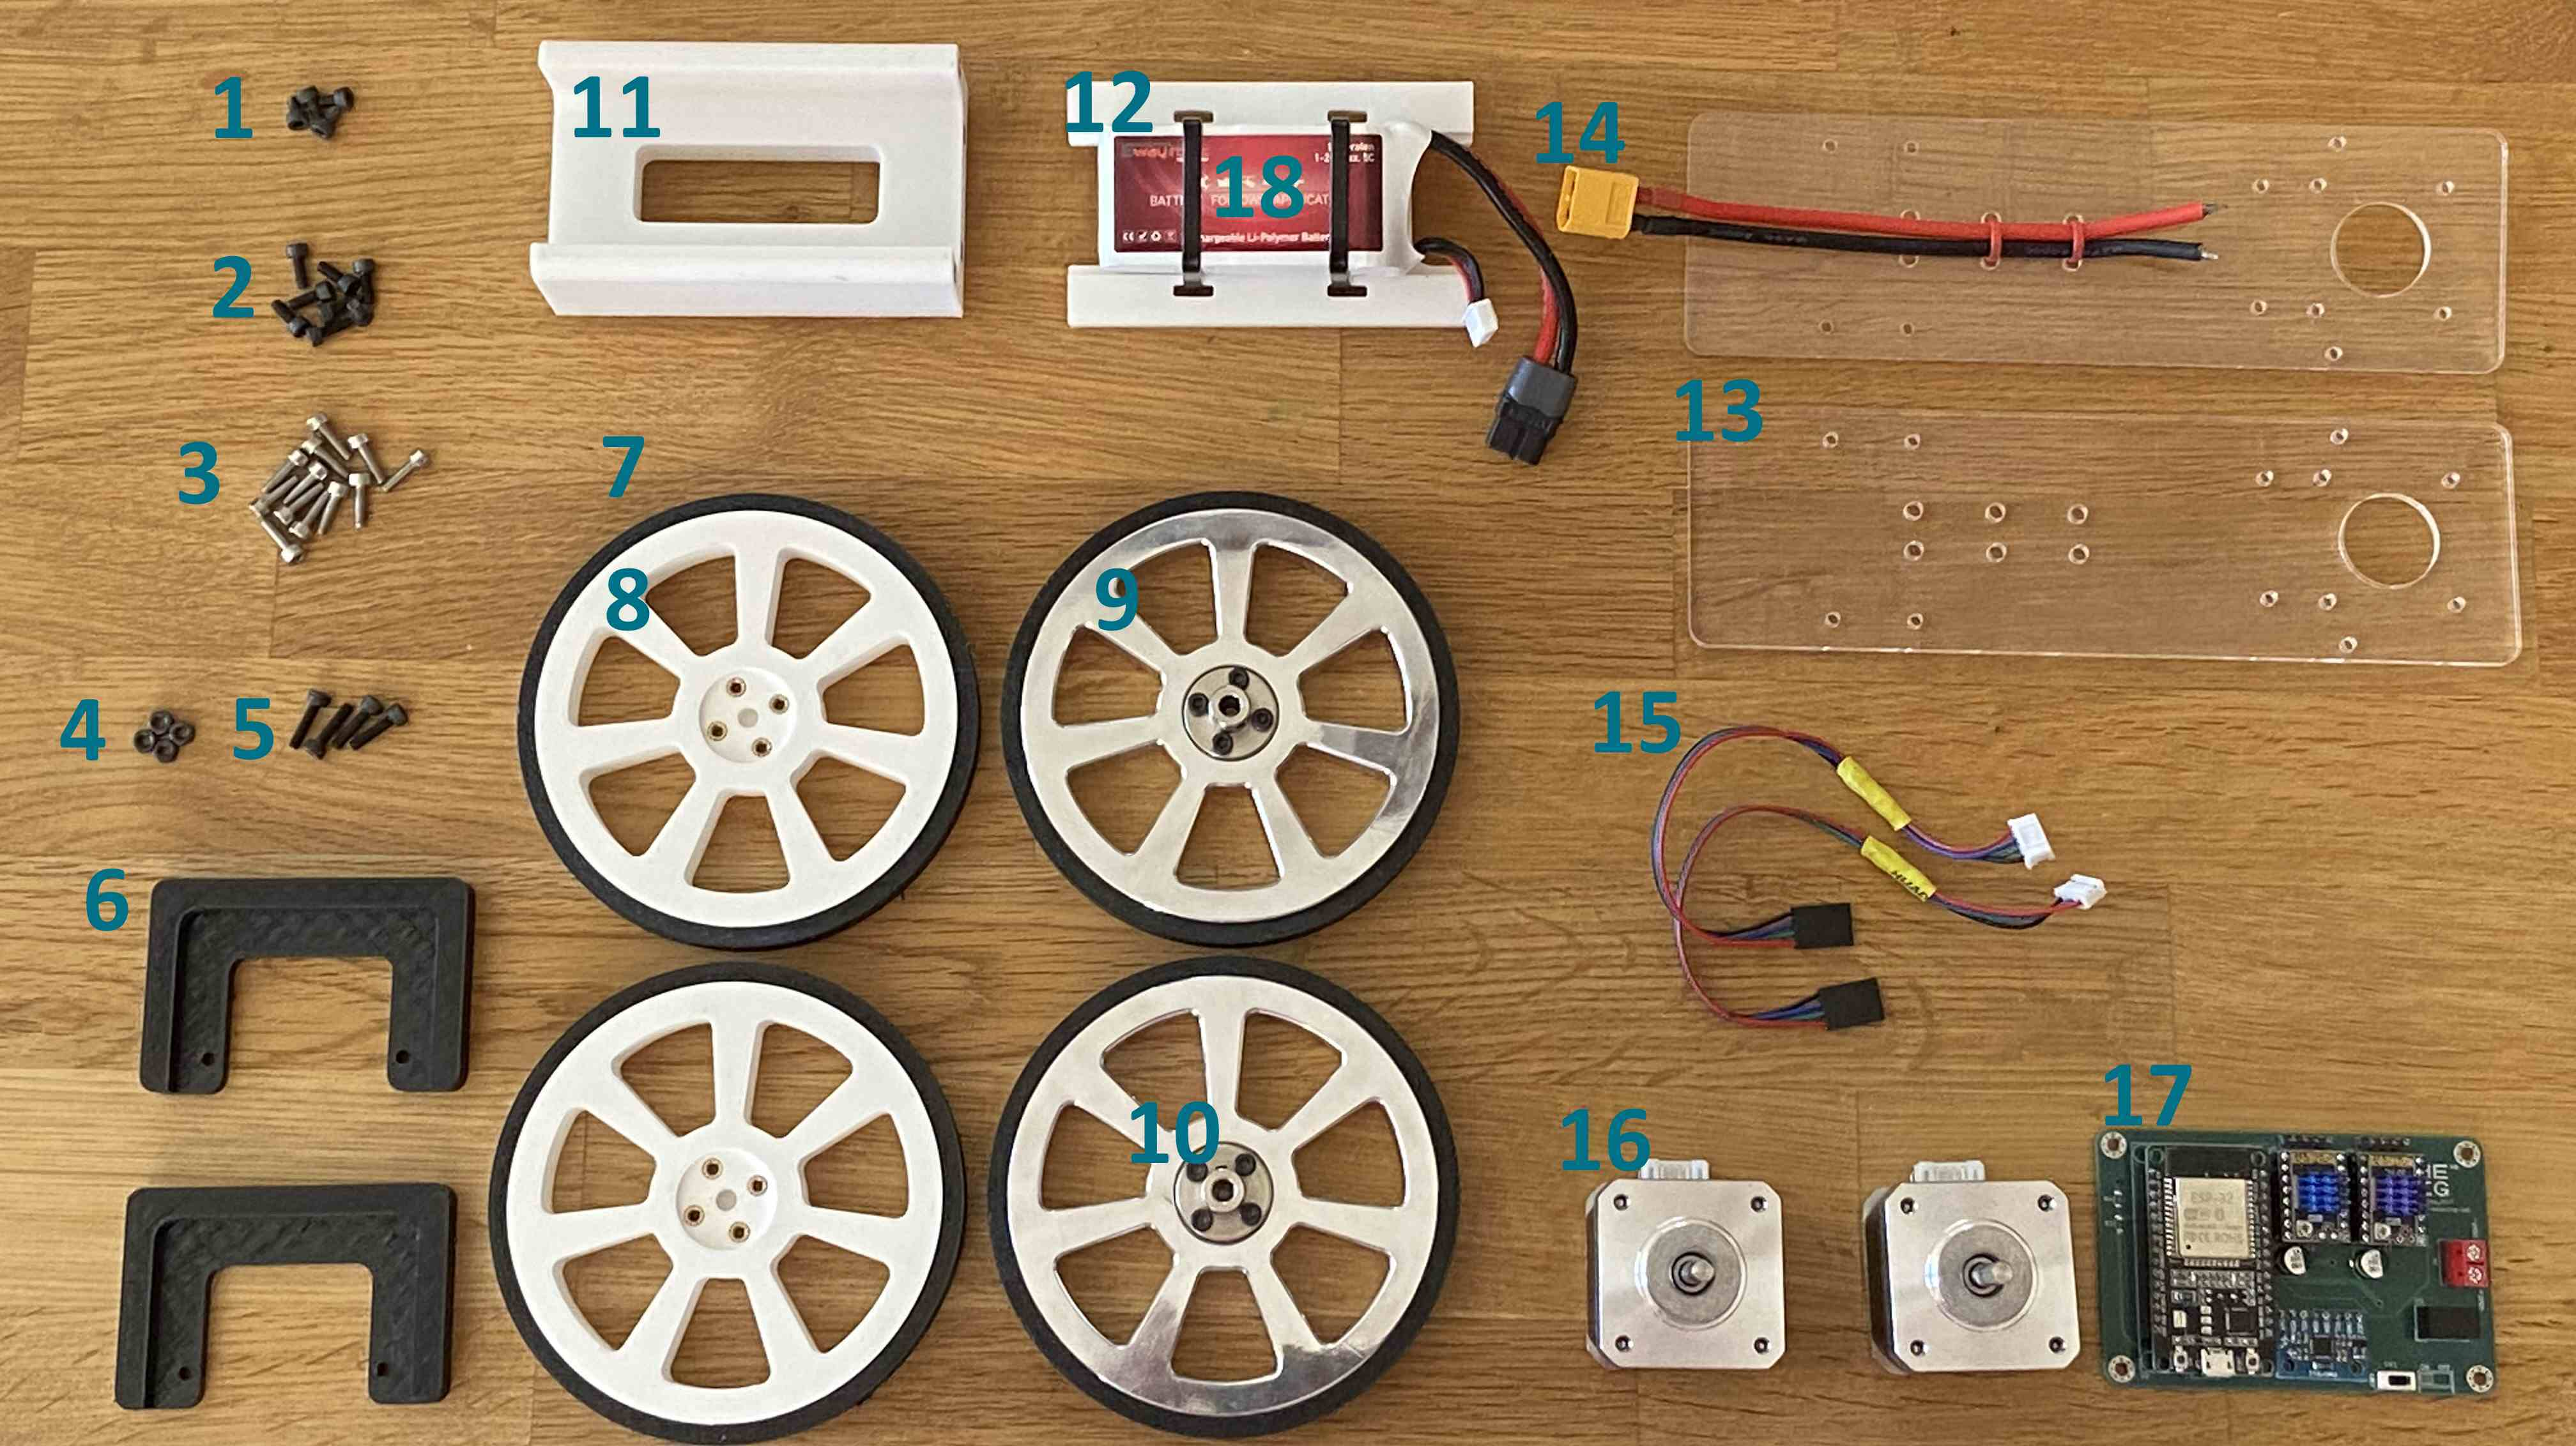
\includegraphics[width=1\textwidth]{assets/figures/all_pieces.jpg}
    \caption{Ensemble des pièces composant la maquette}
    \label{fig:all_pieces}
\end{figure}

Le tableau \ref{tab:masse_pieces} présente les masses individuelles des composants identifiés sur la figure \ref{fig:all_pieces}. Les masses des vis, écrous et inserts M3 sont négligées dans les calculs, leur contribution étant faible devant la masse totale de la maquette.
Les résultats sont donnés en \si{\kilogram}.
\begin{table}[H]
\centering
\begin{tabular}{|c|p{6cm}|c|c|c|}
\hline
\textbf{Pièce} & \textbf{Désignation} & \textbf{Mesure} & \textbf{Fusion360} & \textbf{Unité} \\
\hline
6 & Protection anti-chute & $0.010$ & -- & \si{\kilogram} \\
\hline
7 & Pneu & $0.013$ & $0.014$ & \si{\kilogram} \\
\hline
8 & Jante PLA & $0.035$ & $0.030$ & \si{\kilogram} \\
\hline
9 & Jante ALU & $0.163$ & 0.163& \si{\kilogram} \\
\hline
10 & Coupleur avec vis de montage & $0.013$ & $0.010$ & \si{\kilogram} \\
\hline
11 & Support PCB & $0.047$ & $0.047$ & \si{\kilogram} \\
\hline 
12 & Support batterie& $0.018$ & $0.018$ & \si{\kilogram} \\
\hline
13 & Plaque latérale & $0.065$ & $0.065$ & \si{\kilogram} \\
\hline
14 & Câble d'alimentation & $0.016$ & $-$ & \si{\kilogram} \\
\hline
15 & Câble moteur & $0.000$ & $-$ & \si{\kilogram} \\
\hline
16 & Moteur pas à pas & $0.281$ & 0.281 & \si{\kilogram} \\
\hline
17 & PCB & $0.045$ & 0.045& \si{\kilogram} \\
\hline
18 & Batterie & $0.150$ & 0.150 & \si{\kilogram} \\
\hline
\end{tabular}
\caption{Masses des différentes pièces composant la maquette.}
\end{table}
\label{tab:masse_pieces}

A partir des masses individuelles et des propriétés géométriques obtenues par Fusion360, les paramètres mécaniques nécessaires à la modélisation dynamique (voir \ref{chap:principe_physique}) sont déterminés.

La masse totale des sous-ensembles est obtenue à l'aide d'une nouvelle mesure.

Les moments d'inertie sont directement extraits de Fusion360 à partir de l'outil d'analyse des propriétés de masse. Le calcul est effectué autour du centre de masse du sous-ensemble considéré et selon l'axe de rotation correspondant. Pour les roues, le moment d'inertie $J_w$ est calculé autour de l'axe de rotation de la roue. Pour le châssis, le moment $J_b$ correspond au moment d'inertie autour de l'axe des roues, après exclusion des masses tournantes.

La distance $l$ entre l'axe des roues et le centre de masse est également déterminée à partir de la position du centre de gravité calculée par Fusion360.
\begin{table}[H]
\centering
\begin{tabular}{|l|c|p{5.2cm}|c|c|}
\hline
\textbf{Symbole} & \textbf{Origine} & \textbf{Définition} & \textbf{Valeur} & \textbf{Unité} \\
\hline
$m_b$ & Mesure & Masse du châssis & $1.018$ & \si{\kilogram} \\
\hline
$m_w$ & Mesure & Masse d'une roue complète (coupleur, jante ALU et pneu) & $0.195$ & \si{\kilogram} \\
\hline
$-$ & Mesure & Masse d'une roue complète (coupleur, jante PLA et pneu) & $0.083$ & \si{\kilogram} \\
\hline
$l$ & Fusion360 & Distance entre l'axe des roues et le centre de masse & $0.0344$ & \si{\metre} \\
\hline
$r$ & Mesure & Rayon de la roue & $0.055$ & \si{\metre} \\
\hline
$J_w$ & Fusion360 & Moment d'inertie d'une roue (ALU) autour de son axe de rotation & $2.522\times10^{-4}$ & \si{\kilogram\metre\squared} \\
\hline
$-$ & Fusion360 & Moment d'inertie d'une roue (PLA) autour de son axe de rotation & $7.615\times10^{-5}$ & \si{\kilogram\metre\squared} \\
\hline
$J_b$ & Fusion360 & Moment d'inertie du châssis (sans les roues) autour de l'axe des roues & $4.021\times10^{-3}$ & \si{\kilogram\metre\squared} \\
\hline
\end{tabular}
\caption{Caractéristiques mécaniques de la maquette utilisées dans la modélisation.}
\label{tab:caracteristiques_mecaniques}
\end{table}

L'analyse du modèle CAO réalisée sous Fusion 360 permet de déterminer avec précision la position de l'\acrshort{imu} par rapport à l'axe de rotation des roues. Cette information est nécessaire pour tenir compte des accélérations linéaires mesurées par le capteur lors des mouvements du robot.

La position de l'\acrshort{imu} est exprimée en coordonnées polaires, définies par la distance $\rho$ entre le capteur et l'axe de rotation, ainsi que par l'angle $\phi$ :

$$
\phi = -0.373~\mathrm{rad}
$$

$$
\rho = 51.13~\mathrm{mm}
$$
